%!TEX root = ./template-skripsi.tex
%-------------------------------------------------------------------------------
%                            BAB III
%               			PEMBAHASAN
%-------------------------------------------------------------------------------

\chapter{METODOLOGI PENELITIAN}

\section{Deskripsi Sistem}

Penelitian yang akan dibuat oleh penulis adalah memperbaharui dan melanjutkan penelitian sistem aplikasi yang telah dibuat sebelumnya oleh (Rahmadati, 2023) yang berjudul “PERANCANGAN APLIKASI PENGKAJIAN LUKA KRONIS BERBASIS ANDROID MODUL PENGOLAHAN CITRA” dalam pembuatan aplikasi skoring luka. Aplikasi ini berfungsi sebagai alat untuk membantu perawat dalam mengidentifikasi tingkat penyembuhan luka pasien. Selain hal tersebut, aplikasi ini juga akan diintegrasi dengan sistem pewarnaan luka otomatis (Aprillia, 2021) dan sistem anotasi luka otomatis (Rizki, 2022) serta menambahkan fitur manajemen keperawatan. Penelitian ini juga akan terhubung dengan (Insan, 2023) pada database yang sedang dikembangkan.

Penelitian ini dimulai dengan menganalisis kebutuhan, kemudian lanjut ke proses pengembangan, dan diakhiri dengan pengujian serta evaluasi. Tahapan penelitian yang penulis lakukan dalam penelitian aplikasi ini dapat dilihat pada gambar 3.1.


\begin{figure}[H]
	\centering
	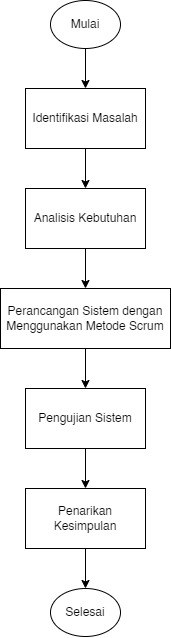
\includegraphics[keepaspectratio, width=4cm]{gambar/tahapan_penelitian}
	\caption{Tahapan Penelitian}
	\label{gambar:tahapan_penelitian}
\end{figure}

\section{Analisa Kebutuhan}

Berdasarkan wawancara dengan bu Ratna pada lampiran A, prioritas fitur pada aplikasi ini terfokus pada kajian luka yang belum ada pada aplikasi sebelumnya (Rahmadati, 2022) yang terdapat pada \textit{Bates-Jensen Wound Assessment Tools} dan fitur manajemen keperawatan serta penambahan user pada pasien. Berikut adalah \textit{usecase} yang telah didefinisikan berdasarkan wawancara.

\begin{figure}[H]
	\centering
	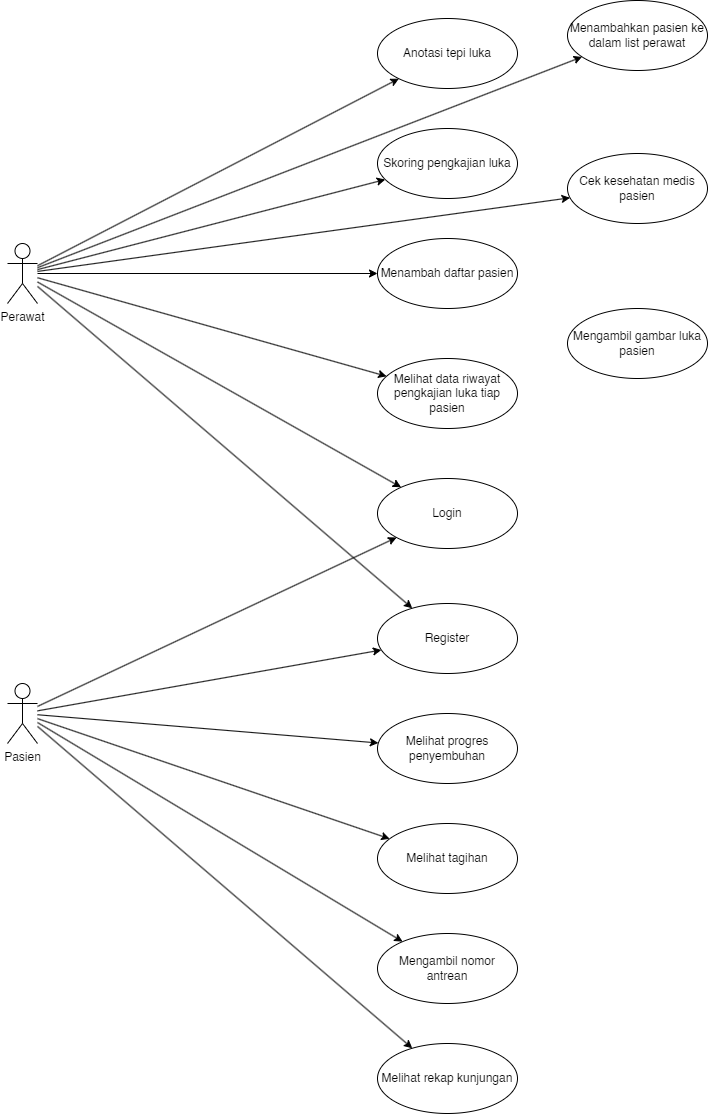
\includegraphics[keepaspectratio, width=8cm]{gambar/usecase}
	\caption{Use Case}
	\label{gambar:use_case}
\end{figure}

Perangkat yang dibutuhkan oleh penulis adalah sebagai berikut:
\begin{enumerate}
\item Laptop dengan spesifikasi minimum dapat menjalankan program aplikasi android studio.
\item Smartphone android untuk uji coba aplikasi ketika selesai.
\item Android Studio sebagai IDE untuk pembuatan aplikasi berbasis Android.
\item Kotlin sebagai bahasa pemrograman penyusun aplikasi.
\item Flask sebagai web framework.
\item MongoDB sebagai basis data.
\item Figma untuk desain tampilan aplikasi.
\end{enumerate}

\section{Perancangan Sistem}

Metode perancangan sistem pada penelitian ini sesuai dengan komponen yang ada di dalam metode \textit{Scrum}. Komponen-komponen tersebut terdiri dari \textit{product backlog, sprint backlog, sprint, daily scrum,} dan pengujian sistem. Tahapan ini dilakukan setelah dilakukannya tahapan analisis kebutuhan.

\begin{figure}[H]
	\centering
	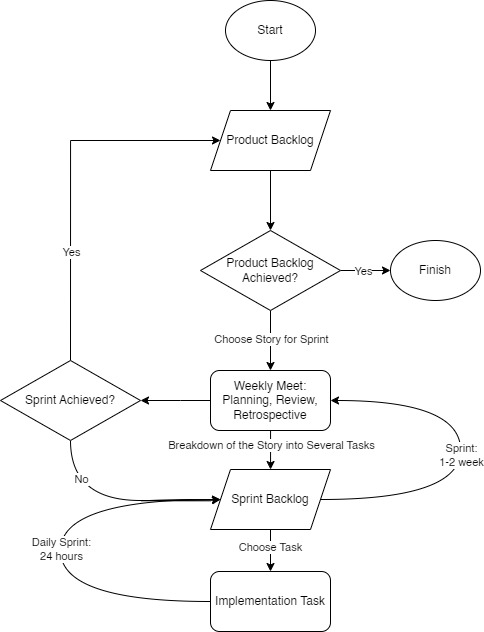
\includegraphics[keepaspectratio, width=10cm]{gambar/metode_scrum}
	\caption{Tahapan Pengembangan Metode Scrum}
	\label{gambar:scrum}
\end{figure}

\begin{enumerate}
\item \textit{Product Backlog}

Product Backlog berisi fitur-fitur yang dibuat berdasarkan kebutuhan pengguna dan sudah didiskusikan dengan Scrum Master. Tabel 3.1 merupakan rincian product backlog dari aplikasi yang akan dibuat.

\begin{table}[H]
	\caption{\textit{Product Backlog}}
	\label{product_backlog}
	\begin{tabular}{@{} |p{0.5cm}|p{7cm}|p{1.5cm}|p{2cm}|p{2cm}| @{}}
		\hline
		\textbf{No} & \textbf{\textit{User Story}} & \textbf{\textit{Role}} & \textbf{\textit{Priority}} & \textbf{\textit{Sprint}} \\
		\hline
		1 & \textit{Skoring Bates-Jensen} & Perawat & High & \multirow{5}{2cm}{1} \\
		\cline{1-4}
		2 & Konversi seluruh activity menjadi fragment & & High &  \\
		\cline{1-4}
		3 & Login user & Perawat, Pasien & High &  \\
		\hline
		4 & Evaluasi kondisi kesehatan pasien sebelum perawatan & Perawat & High & 2 \\
		\hline
		5 & Catatan perkembangan/ diagnosis untuk langkah penyembuhan selanjutnya & Perawat & High & 3 \\
		\hline
		6 & Rekap kunjungan pasien & Perawat & High & 4 \\
		\hline
		7 & Implementasi web service program warna luka & Perawat & Low & \multirow{4}{2cm}{5} \\
		\cline{1-4}
		8 & Implementasi web service anotasi luka & Perawat & Low &  \\
		\cline{1-4}
		9 & Mengembangkan progres penyembuhan luka pasien penelitian sebelumnya & Perawat & Low &  \\
		\hline
		10 & \textit{Wound History} & Perawat & High & 6 \\
		\hline
		11 & Registrasi akun pasien & Pasien & Low & \multirow{4}{2cm}{7} \\
		\cline{1-4}
		12 & Mengambil nomor antrean & Pasien & Low &  \\
		\cline{1-4}
		13 & Melihat rekap kunjungan & Pasien & Low &  \\
		\cline{1-4}
		14 & Melihat histori kajian & Pasien & High &  \\
		\hline
		15 & Inventaris & Perawat & Low & 8 \\
		\hline
		16 & Menambah pasien ke dalam akun perawat & Perawat & Low & 9 \\
		\hline
	\end{tabular}
\end{table}
Berdasarkan tabel di atas, Product Backlog pada penelitian ini terdiri dari 5 komponen yaitu: User Story, Role, Sprint, Status. User Story berisi fitur-fitur besar yang akan dibuat pada aplikasi ini. Komponen role pada tabel ini menandakan siapa yang menggunakan fitur tersebut. Priority menentukan tingkat prioritas dari sebuah User Story. Sprint menandakan informasi urutan fitur yang akan dibuat. Dan status menjelaskan apakah fitur tersebut sudah selesai atau belum.

\item Sprint Backlog

Sprint Backlog adalah daftar task yang perlu dikerjakan ataupun yang sudah dikerjakan pada sprint. Di dalam sprint backlog, berbagai task kecil dibuat. Dengan sprint backlog, seluruh anggota tim dapat melihat perkembangan dari setiap pekerjaan.

\item Sprint

Setelah dilakukan perencanaan pada Sprint Backlog, maka pengerjaan sprint sudah dapat dimulai dan harus mengikuti jadwal pengerjaan yang telah disepakati bersama tim. Dalam penelitian ini, interval sprint yang digunakan adalah satu sampai dua minggu. Berikut merupakan laporan hasil Sprint-1.
	
	
\item Sprint Review dan Sprint Retrospective
	
Sprint review dan sprint retrospective dilakukan pada setiap wal pekan yaitu di hari Selasa melalui daring menggunakan platform discord dan tatap muka secara langsung di UNJ. Pada awal pekan ini akan dilakukan evaluasi mengenai perkembangan proses pembuatan aplikasi maupun hambayan yang terjadi selama pengerjaan di setiap sprint.
	
\item Deploy
	
Pada tahap ini peneliti akan melakukan uji aplikasi pengkajuan luka kronis menggunakan dua jenis pengujian yaitu unit testing dan user acceptance test (UAT). Pengujian unit testing dilaksanakan oleh tim internal developer untuk memastikan fungsi-fungsi pada aplikasi yang telah dikembangkan dapat berjalan dengan baik. Sedangkan UAT dilaksanakan oleh pengguna yang mengetahui apakah aplikasi sudah sesuai kebutuhan dan layak untuk diuji secara masif.
\end{enumerate}

\section{Pengujian}

Pada tahap ini peneliti akan melakukan uji aplikasi pengkajuan luka kronis menggunakan dua jenis pengujian yaitu unit testing dan user acceptance test (UAT). Pengujian unit testing dilaksanakan oleh tim internal developer untuk memastikan fungsi-fungsi pada aplikasi yang telah dikembangkan dapat berjalan dengan baik. Sedangkan UAT dilaksanakan oleh pengguna yang mengetahui apakah aplikasi sudah sesuai kebutuhan dan layak untuk diuji secara masif.

\begin{enumerate}
\item Unit Testing

Skenario pada unit testing dibuat berdasarkan product backlog. Adapun skenario dari unit testing yang akan dilaksanakan terdapat pada tabel 3.3.
	
	\begin{longtable}[c]{@{} |p{4cm}|p{9.3cm}| @{}}
 	\caption{Skenario \textit{Unit Testing} \label{unit_testing}}\\

 	\hline
 	\multicolumn{2}{| c |}{\textbf{Skenario \textit{Unit Testing}}}\\
 	\hline
 	\centering{\textbf{Uji Fitur}} & \centering{\textbf{Skenario Pengujian}}  
 	\endfirsthead

 	\hline
 	\multicolumn{2}{| c |}{\textbf{Skenario \textit{Unit Testing}}}\\
 	\hline
 	\centering{\textbf{Uji Fitur}} & \centering{\textbf{Skenario Pengujian}}
 	\endhead

 	\hline
 	\endfoot

 	\hline
 	\endlastfoot

 	\hline
 	
 	Halaman Awal & Saat aplikasi dibuka akan muncul tampilan awal dengan pilihan "Login" dan "Register"\\
	\hline
	& Jika tombol "Login" ditekan, guest akan masuk ke halaman Login\\
	\hline
	& Jika tombol "Register" ditekan, guest akan masuk ke halaman Register\\
	\hline
	Register & Ketika mengisi form registrasi dengan lengkap kemudian submit, maka akan kembali ke halaman Login\\
	\hline
	& Ketika mengisi form registrasi tidak lengkap kemudian submit, maka akan menampilkan pesan kesalahan untuk melengkapi data yang kosong\\
	\hline
	Login & Ketika mengisi form login dengan data yang tidak sesuai kemudian klik submit, maka akan menampilkan pesan kesalahan username atau password\\
	\hline
	& Ketika mengisi form login dengan data yang sesuai dengan role perawat, maka akan masuk ke halaman beranda perawat\\
	\hline
	& Ketika mengisi form login dengan data yang sesuai dengan role pasien, maka akan masuk ke halaman beranda pasien\\
	\hline
	Beranda Perawat & Saat ikon profil pada kanan atas di-klik maka akan muncul halaman profil perawat\\
	\hline
	& Saat tombol daftar pasien di-klik maka akan muncul halaman daftar pasien\\
	\hline
	& Saat tombol pewarnaan luka ditekan, maka akan muncul halaman pewarnaan luka otomatis\\
	\hline
	& Saat tombol medical record ditekan, maka akan muncul halaman medical record pasien\\
	\hline
	Tambah hasil kajian & Saat pertama kali klik tombol tambah kajian baru muncul halaman pemeriksaan kesehatan pasien sebelum perawatan\\
	\hline
	& Ketika mengisi form pemeriksaan kesehatan dengan tidak lengkap maka akan menampilkan pesan kesalahan bahwa data yang diisi kurang sesuai atau belum lengkap\\
	\hline
	& Ketika mengisi form pemeriksaan kesehatan dengan lengkap maka akan masuk ke halaman ambil foto luka\\
	\hline
	& Ketika pengguna menekan tombol kamera, maka akan masuk ke halaman pengambilan foto luka\\
	\hline
	& Ketika pengguna selesai mengambil foto luka, maka akan diarahkan ke halaman anotasi tepi luka otomatis.\\
	\hline
	& Ketika anotasi tepi luka otomatis selesai bekerja, maka pengguna dapat menekan tombol "SAVE" untuk lanjut ke halaman kajian luka atau tekan tombol "EDIT" untuk menganotasi luka secara manual.\\
	\hline
	& Ketika mengisi form kajian luka secara tidak lengkap kemudian klik "NEXT", maka akan muncul pesan kesalahan bahwa data yang diisi belum lengkap\\
	\hline
	& Ketika mengisi form kajian luka secara lengkap kemudian klik "NEXT", maka akan diarahkan ke halaman tujuan perawatan.\\
	\hline
	& Ketika mengisi form tujuan perawatan secara tidak lengkap kemudian klik submit, maka akan muncul pesan kesalahan bahwa data yang diisi belum lengkap\\
	\hline
	& Ketika mengisi form tujuan perawatan secara lengkap kemudian klik submit, maka akan diarahkan ke halaman detail pasien yang baru saja diinput\\
	\hline
	Detail pasien & Saat masuk pertama kali ke halaman detail pasien, maka akan muncul informasi umum pasien dan progres tingkat kesembuhan luka pasien berdasarkan skoring kajian luka sebelumnya\\
	\hline
	& Saat tab Histori Kajian diklik maka akan muncul histori kajian pasien dan progres tingkat kesembuhan luka pasien berdasarkan skoring kajian luka sebelumnya\\
	\hline
	Beranda Pasien & Saat ikon profil pada kanan atas di-klik maka akan muncul halaman profil pasien\\
	\hline
	& Saat tombol riwayat kajian luka ditekan, maka akan muncul halaman riwayat kajian luka pasien\\
	\hline
	& Saat tombol rekap kunjungan ditekan, maka akan muncul halaman rekap kunjungan pasien\\
	\hline
	& Saat tombol medical record ditekan, maka akan muncul halaman medical record pasien\\
	\hline
	Profil Pasien & Saat ikon profil pada kanan atas di-klik maka akan muncul halaman profil pasien\\
	\hline
	& Saat tombol ambil antrean ditekan, maka akan diarahkan ke halaman antrean.\\
	\hline
	& Saat tombol riwayat kajian luka ditekan, maka akan muncul halaman riwayat kajian luka pasien.\\
	\hline
	& Saat tombol rekap kunjungan ditekan, maka akan muncul halaman rekap kunjungan pasien.\\
	\hline
	& Saat tombol medical record ditekan, maka akan muncul halaman medical record pasien.\\
	\hline
	Antrean & Saat masuk pertama kali ke halaman antrean, maka akan muncul nomor antrean saat ini, nama, nomor registrasi dan tombol ambil antrean.\\
	\hline
	& Saat tombol antrean ditekan, maka akan muncul nomor antrean yang diambil lalu tombol ambil antrean berubah menjadi selesai berobat.\\
	\hline
	& Saat tombol selesai berobat ditekan maka tombol tersebut akan menghilang lalu diarahkan kembali ke halaman beranda.\\
	\hline
	Riwayat kajian luka & Saat ikon profil pada kanan atas di-klik maka akan muncul halaman profil pasien\\
	\hline
	& Saat tombol riwayat kajian luka ditekan, maka akan muncul halaman riwayat kajian luka pasien\\
	\hline
	& Saat tombol rekap kunjungan ditekan, maka akan muncul halaman rekap kunjungan pasien\\
	\hline
	& Saat tombol medical record ditekan, maka akan muncul halaman medical record pasien\\
	\hline
	Rekap kunjungan & Saat ikon profil pada kanan atas di-klik maka akan muncul halaman profil pasien\\
	\hline
	& Saat tombol riwayat kajian luka ditekan, maka akan muncul halaman riwayat kajian luka pasien\\
	\hline
	& Saat tombol rekap kunjungan ditekan, maka akan muncul halaman rekap kunjungan pasien\\
	\hline
	& Saat tombol medical record ditekan, maka akan muncul halaman medical record pasien\\
	\hline
 	\end{longtable}
 	
\item User Acceptance Testing

Skenario dalam Uji Penerimaan Pengguna disusun berdasarkan fitur-fitur yang dapat diakses oleh pengguna dalam backlog produk. Detail skenario UAT yang akan dilaksanakan tercantum dalam tabel 3.4.

\begin{longtable}[c]{@{} |p{4cm}|p{7cm}|p{2.3cm}| @{}}
 	\caption{Skenario \textit{Unit Acceptance Testing} \label{unit_acceptance_testing}}\\

 	\hline
 	\centering{\textbf{Uji Fitur}} & \centering{\textbf{Skenario Pengujian}} & \centering{\textbf{Jenis Pengujian}}
 	\endfirsthead

 	\hline
 	\centering{\textbf{Uji Fitur}} & \centering{\textbf{Skenario Pengujian}} & \centering{\textbf{Jenis Pengujian}}
 	\endhead

 	\hline
 	\endfoot

 	\hline
 	\endlastfoot

 	\hline
 	
 	Registrasi & Menekan tombol buat akun lalu mengisi 
form registrasi kemudian submit & UAT\\
	\hline
	Login & Menekan tombol login lalu mengisi form login dengan NIP dan password kemudian submit & UAT\\
	\hline
	Daftar pasien & Klik tombol daftar pasien pada beranda kemudian menampilkan daftar pasien & UAT\\
	\hline
	Melihat detail pasien & Klik tombol daftar pasien pada beranda kemudian klik pasien yang ingin dilihat detailnya & UAT\\
	\hline
	Galeri luka & Klik tombol galeri luka kronis pada beranda & UAT\\
	\hline
	Arsir warna luka & Klik tombol arsir warna luka kronis pada beranda kemudian unggah gambar melalui galeri lalu mengarsir warna luka dan submit & UAT\\
	\hline
	Menambahkan kajian luka baru & Buka halaman detail pasien lalu klik tab histori kajian luka kemudian klik tombol tambah hasil kajian dilanjutkan dengan isi form kajian dan submit & UAT\\
	\hline
	Anotasi tepi luka & Buka halaman detail pasien lalu klik tab histori kajian luka kemudian klik icon tambah dilanjutkan dengan memfoto luka kronis lalu melakukan anotasi tepi luka dan submit & UAT\\
	\hline
	Anotasi diameter luka & Setelah melakukan anotasi tepi luka, masuk ke halaman anotasi diameter luka kemudian melakukan anotasi diameter luka dan submit & UAT\\
	\hline
	Melihat histori kajian luka & Buka halaman detail pasien lalu klik tab histori kajian luka & UAT\\
	\hline
	Melihat detail dari histori kajian luka & Buka halaman detail pasien lalu klik tab histori kajian luka kemudian klik card sesuai dengan tanggal kajian luka yang ingin dilihat & UAT\\
	\hline
	Galeri luka satu pasien & Buka halaman detail pasien lalu klik tab galeri luka pasien & UAT\\
	\hline
	Profil perawat & Dari halaman beranda, klik ikon profil pada kanan atas & UAT\\
	\hline
	Logout & Pada halaman profil perawat, klik tombol logout & UAT\\
	\hline
 	\end{longtable}
\end{enumerate}


%\subsection{\textit{Daily Scrum}}

%Pada akhir pekan di akhir setiap \textit{sprint}, akan diadakan \textit{voice call} untuk membahas perkembangan dan hambatan pada setiap \textit{sprint}.